\documentclass{article}

%Librerías
\usepackage[utf8]{inputenc}
\usepackage[spanish,mexico]{babel}
\setlength{\textwidth}{18cm}
\setlength{\oddsidemargin}{-1cm}
\setlength{\headsep}{-1cm}
\setlength{\voffset}{0cm}
\setlength{\topmargin}{0cm}
\setlength{\headheight}{0cm}
\usepackage{tikz}
\usetikzlibrary{calc,arrows}
\usepackage{multicol}
\usepackage{lipsum} 
%\bibliographystyle{apacite}
\usepackage[spanish]{babel}
\selectlanguage{spanish}


\begin{document}

%%%%%% ENCABEZADO %%%%%%%%%%%%%%%%%%%%%%%%%%%%%%%%%%%%%%%
% Logo de la maestría
\colorbox{white!10!}{
    \begin{minipage}[t]{0.05\textwidth} %0.165 
       \begin{flushright}
        
\includegraphics[width=2in]{logo UPS.png}
       \end{flushright}
    \end{minipage}
    \begin{minipage}[H]{0.62 \textwidth} %0.62
        \begin{center}
         
        \end{center}
     \end{minipage}
    \begin{minipage}[t]{0.05 \textwidth}
        \begin{flushleft}
        \hspace{10.25cm}
            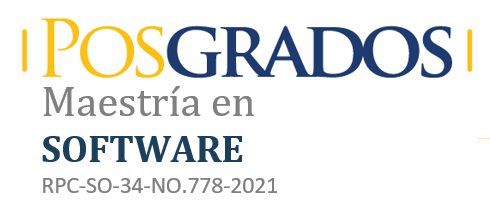
\includegraphics[width=2in]{Posgrados.png}
        \end{flushleft}
    \end{minipage}
}

\begin{tikzpicture}
    \draw[thick] (-6.5,0)--(11.2,0);
\end{tikzpicture}
%%%%%%%%%%%%%%%%%%%%%%%%%%%%%%%%%%%%%%%%%%%%%%%%%%%%%%%%%
\vspace{0.1cm}
\begin{center}
{\large\textsc{ANTEPROYECTO DEL TRABAJO DE TITULACIÓN}} \\
\vspace{0.5cm}
{ \large \textbf{Bryam Fernando Cabrera}} \\ 
\vspace{0.25cm}
{ \large \textbf{Willian Ariolfo  Lituma}}
\end{center}
\vspace{0.1cm}

\section{Tema del Trabajo de Titulación:  }
\begin{center}
Análisis, Desarrollo y Migración a un nuevo sistema contable para la empresa Accescont 
\end{center}
\section{Docente tutor propuesto:   }
\begin{center}
Asignar Tutor
\end{center}
\section{Antecedentes}

En el actual entorno empresarial, la tecnología de la información y los sistemas contables desempeñan un papel fundamental en el éxito y la eficiencia de las organizaciones. En este contexto, Accescont, una destacada firma de auditoría financiera con sede en Cuenca, Ecuador, se enfrenta a desafíos significativos debido a las limitaciones y obsolescencia de su sistema contable actual. Este sistema ha quedado rezagado en términos de funcionalidades y seguridad, lo que dificulta su capacidad para adaptarse a las crecientes necesidades de la empresa y la incorporación de nuevos módulos contables.

El principal problema de este sistema es su arquitectura monolítica, que ha sido objeto de modificaciones a lo largo de los años para satisfacer las necesidades cambiantes de la empresa. Sin embargo, estas modificaciones han llevado a una degradación significativa del código, lo que podría comprometer el sistema en caso de necesitar más cambios. En consecuencia, la empresa se ha visto en la necesidad de implementar un nuevo sistema de manera ágil, sin afectar a sus clientes.

El proyecto propuesto tiene como objetivo encontrar una solución integral y efectiva para fortalecer las operaciones contables de Accescont, especialmente en los módulos de clientes y proveedores. Esto se logrará mediante la implementación de nuevas herramientas, como los microservicios, que optimizarán la gestión financiera y contribuirán al crecimiento sostenible de la empresa. Además, este enfoque permitirá el escalado del sistema contable y posibles ampliaciones a otros módulos del sistema.

Es importante destacar que el éxito de este proyecto de titulación depende en gran medida del trabajo colaborativo con los usuarios y las partes interesadas de Accescont, así como del cumplimiento de plazos y la ejecución efectiva de las fases planificadas. 

 %\lipsum[1-1]
       
 \section*{\textbf{Justificación del Tema de Trabajo de Titulación}}

 \begin{enumerate}
     \item \textbf{Contexto y Relevancia:} En el contexto empresarial actual, la tecnología de la información y los sistemas contables desempeñan un papel crítico para el éxito y la eficiencia de las organizaciones. Accescont, una firma de auditoría financiera con más de 35 años de experiencia con sede en Cuenca, Ecuador, se enfrenta a desafíos significativos debido a las limitaciones y la obsolescencia de su sistema contable actual. Este sistema, que ha sido parte integral de la empresa durante años, ha quedado rezagado en términos de funcionalidad y seguridad, lo que dificulta su capacidad para adaptarse a las cambiantes necesidades empresariales y la incorporación de nuevos módulos contables.
 
     \item \textbf{Problema de la Arquitectura Monolítica:} El principal problema radica en la arquitectura monolítica del sistema actual, que ha experimentado modificaciones a lo largo del tiempo para satisfacer las necesidades cambiantes de la empresa. Sin embargo, estas modificaciones han llevado a una degradación significativa del código, lo que podría comprometer aún más el sistema en caso de necesitar más cambios. Como resultado, la empresa reconoce la necesidad urgente de implementar un nuevo sistema contable sin afectar a sus clientes existentes.
 
     \item \textbf{Objetivos del Proyecto:} El proyecto propuesto se enmarca en la búsqueda de una solución integral y efectiva para fortalecer las operaciones contables de Accescont, especialmente en los módulos de clientes y proveedores. Se busca superar los desafíos tecnológicos actuales mediante la implementación de nuevas herramientas, como los microservicios, que optimizarán la gestión financiera y contribuirán al crecimiento sostenible de la empresa. Además, este enfoque permitirá el escalado del sistema contable y posibles expansiones a otros módulos del sistema.
 
     \item \textbf{Colaboración y Cumplimiento de Plazos:} Es importante destacar que el éxito de este proyecto de titulación dependerá en gran medida de la colaboración efectiva con los usuarios y las partes interesadas de Accescont. También se hará hincapié en el cumplimiento de los plazos y la ejecución eficiente de las fases planificadas para garantizar la implementación exitosa del nuevo sistema.
 
 \end{enumerate}
 
 En resumen, este trabajo de titulación busca abordar una problemática real en el ámbito empresarial. Accescont se enfrenta a desafíos tecnológicos y de usabilidad con su sistema contable actual, y el proyecto propuesto tiene como objetivo superar estos desafíos mediante la implementación de una solución innovadora y escalable. La colaboración con los stakeholders y el cumplimiento de los plazos son elementos clave para el éxito de este proyecto y su contribución al crecimiento y competitividad de Accescont en el mercado. 

\section{Objetivos:}
Presenta el objetivo general del trabajo y los objetivos específicos que se alcanzarán con el desarrollo del mismo. 
\subsection*{Objetivo General:}
Analizar, desarrollar y migrar  los modulos de clientes y proveedores del sistema contable de la empresa Accescont de la ciudad de Cuenca cambiando su sistema actual por uno de naturaleza modular para agilizar su escalabilidad.
\subsection*{Objetivos Específicos:}

\begin{itemize}
    \item Construir ....
    \item Diseñar ....
\end{itemize}

\section{Alcance:}
El proyecto consiste en Analizar, desarrollar y migrar los módulos de clientes y proveedores del sistema contable de la empresa Accescont de la ciudad de Cuenca, que luego de las pruebas y validaciones necesarias sea implementado en conjunto los demás módulos planeados para el sistema contable de la empresa. Por lo antes expuesto este proyecto únicamente cubrirá los módulos de clientes y proveedores para los cuales se hará una revisión e identificación de requisitos, construcción, migración de datos, pruebas y evaluación.
\section{Metodología:}

Describe de manera clara el método empleado para cumplir los objetivos a través de las actividades dentro de la investigación. 
\section{Cronograma de actividades:}
Detalla las actividades generales que se desarrollarán hasta la fecha en la que el estudiante presentará su Trabajo de Titulación. 

\section{Presupuesto: (Opcional)}

Este apartado incluirá los recursos e información financiera para el Trabajo de Titulación. 
\bibliographystyle{abbrv}
%apacite



\bibliography{sample}

\vspace{1cm}
Este apartado contiene el listado de referencias empleadas para la elaboración del documento, de preferencia en formato APA u otros formatos Preconocidos.


\end{document}
